\section{Impact Factors}\label{impact-factors}

\subsection{Citations}\label{citations}

My overall publication impact was analyzed by using the citation reports
of Clarivate's Web of Science, Elsevier's Scopus, and Google Scholar,
according to the profiles and reports summarized in Table 1 and Figures
1, 2 and 3. My 10 most cited publications and corresponding citations in
the last few years are shown in Figure 4.

Table 1 -- Profiles and citation metrics in Web of Science, Scopus, and
Google Scholar.

\begin{longtable}[]{@{}
  >{\raggedright\arraybackslash}p{(\columnwidth - 6\tabcolsep) * \real{0.2500}}
  >{\raggedright\arraybackslash}p{(\columnwidth - 6\tabcolsep) * \real{0.2500}}
  >{\raggedright\arraybackslash}p{(\columnwidth - 6\tabcolsep) * \real{0.2500}}
  >{\raggedright\arraybackslash}p{(\columnwidth - 6\tabcolsep) * \real{0.2500}}@{}}
\toprule\noalign{}
\begin{minipage}[b]{\linewidth}\raggedright
\end{minipage} & \begin{minipage}[b]{\linewidth}\raggedright
Web of Science
\end{minipage} & \begin{minipage}[b]{\linewidth}\raggedright
Scopus
\end{minipage} & \begin{minipage}[b]{\linewidth}\raggedright
Google Scholar
\end{minipage} \\
\midrule\noalign{}
\endhead
\bottomrule\noalign{}
\endlastfoot
Profile & G-1316-2010 & 7003407125 & auFmh9MAAAAJ \\
Report (27/07/2023) &
\url{https://drive.google.com/file/d/1hlkSJCjBu8D3v9_0Wbu6doJAYw7LKtcr/view?usp=sharing}
&
\url{https://drive.google.com/file/d/1htk2NB3StvbmR1v1UvC81yPWpuaxZbX4/view?usp=sharing}
&
\url{https://drive.google.com/file/d/1hjxngDIEB62qJCfri5TclwdJzn6aqNF8/view?usp=sharing} \\
Number of articles with citation data & 269 & 296 & 401 \\
Number of citations & 3133 & 4686 & 7875 \\
Number of citations excluding self-citations & 2637 & NA & NA \\
\textbf{h-index} & \textbf{24} & \textbf{30} & \textbf{42} \\
\end{longtable}

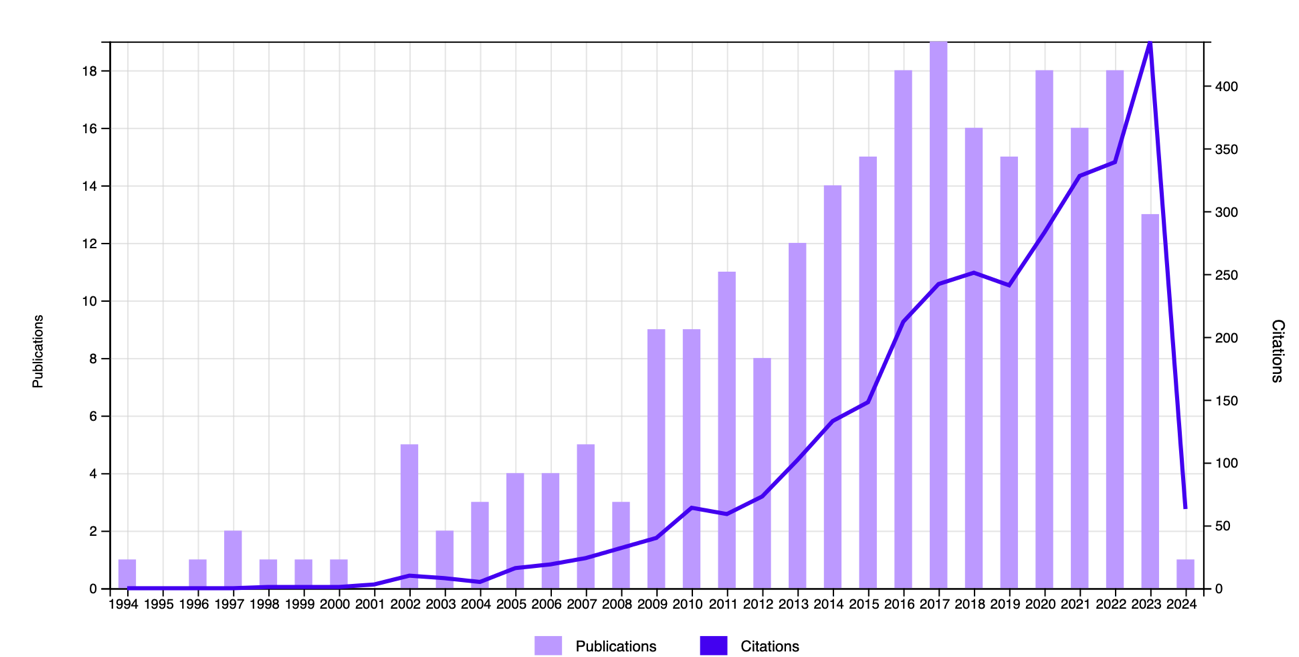
\includegraphics[width=5.90181in,height=2.98425in]{media/image3.png}

Figure 1 -- Web of Science: Citations and publications over time

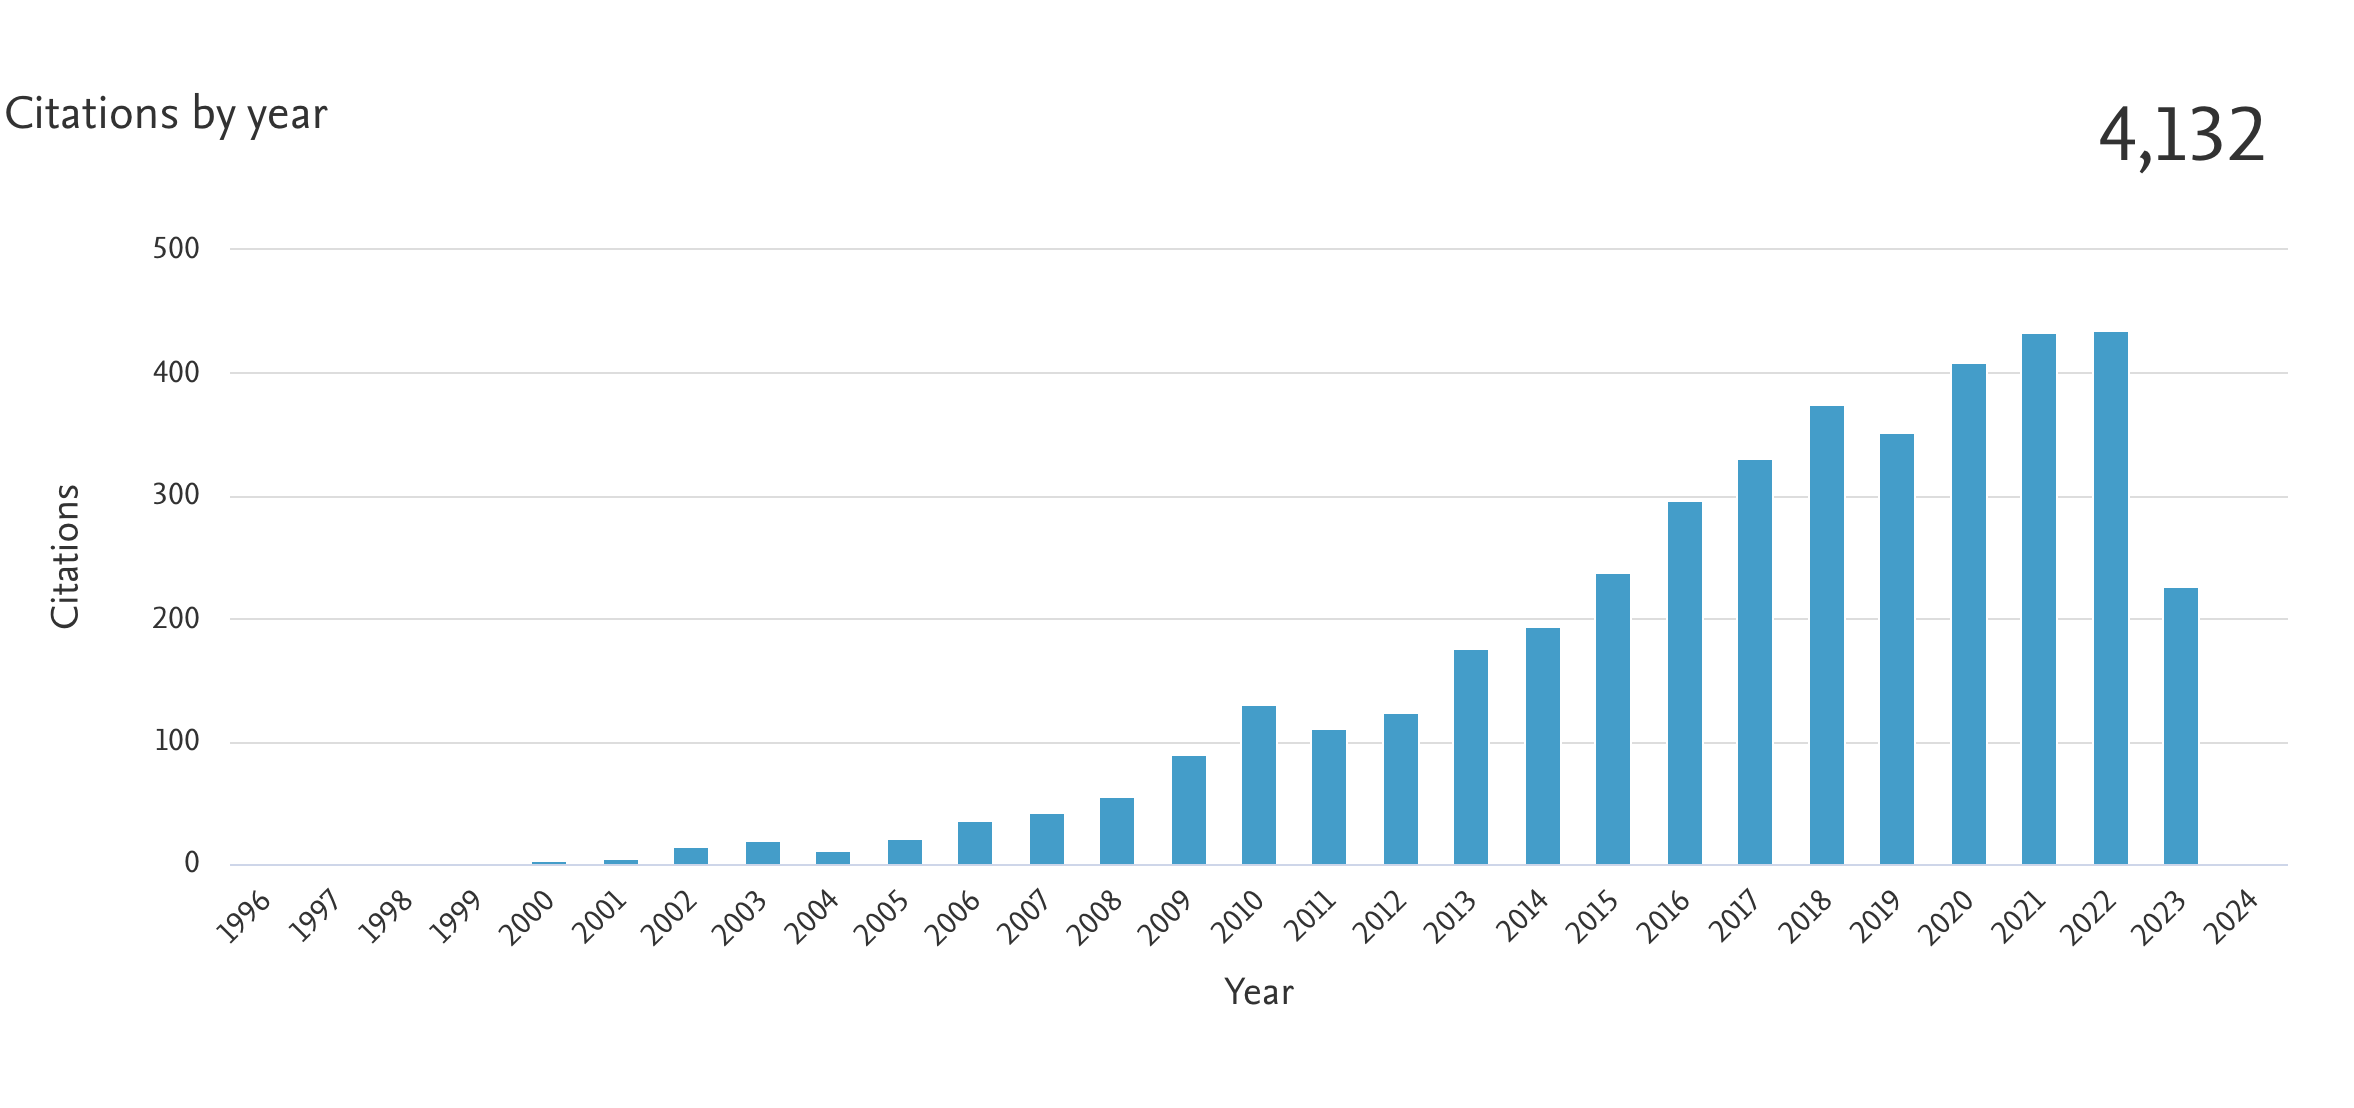
\includegraphics[width=5.75861in,height=2.71024in]{media/image4.png}

Figure 2 -- Scopus : Citations per year

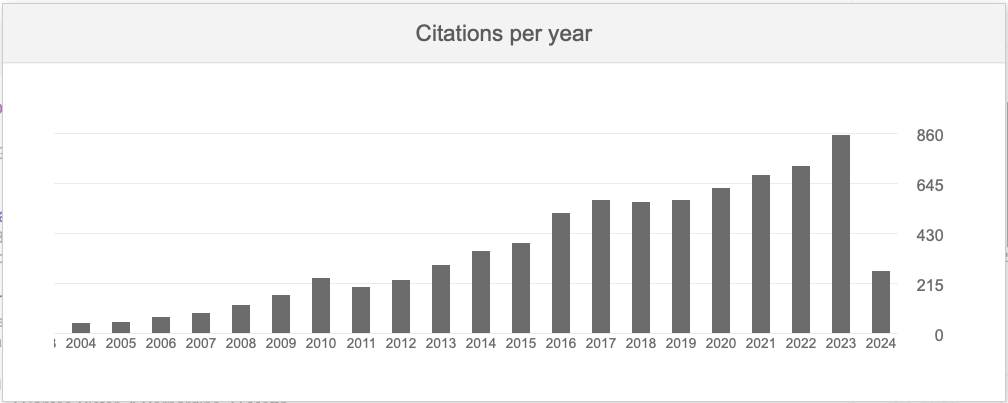
\includegraphics[width=6.06461in,height=2.29217in]{media/image5.png}

Figure 3: Google Scholar: Citations per year.

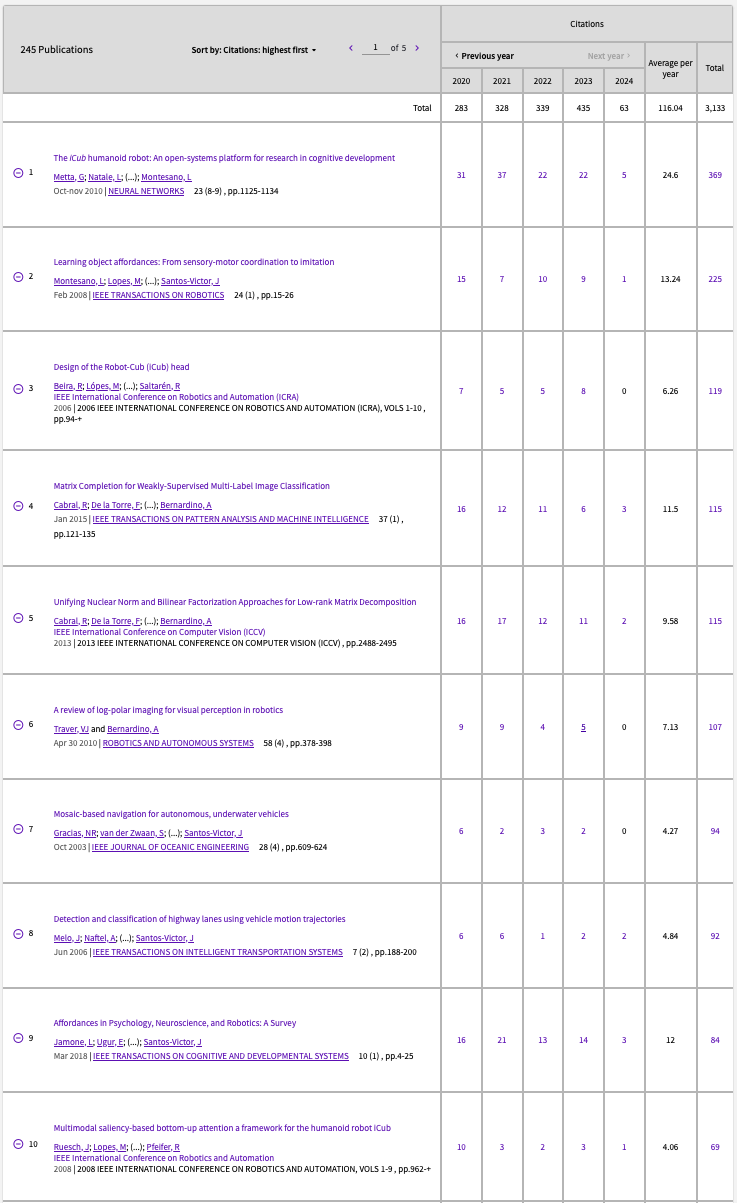
\includegraphics[width=5.76988in,height=9.41831in]{media/image6.png}

Figure 4 -Web of Science : 10 most cited publications.

\subsection{Journal Impact Factors}\label{journal-impact-factors}

Scientific journals are indexed in services that account for several
impact indicators that are typically computed from the number of
citations received by the journal's published articles. Two of the most
renowned journals ranking services are Clarivate Analytics\footnote{Formerly
  known as The Institute for Scientific Information (ISI).} Web of
Science Journal Citation Reports (JCR) and the SCImago Lab's Journal \&
Country Rank (SJR). These services use different types of metrics to
access the relative importance of a journal within its field. Although
there is a large debate about the use of these indexes to assess
scientific work, they carry some value to broadly consider the quality
of the reviewing process in the different journals.

The journals where my papers have been published are listed in Table 2.
For each journal we include the following metrics, when available,
obtained from the Journal Citation Reports (JCR) and the SCImago Journal
Ranks (SJR):

\begin{itemize}
\item
  The 2022 Journal Impact Factor (JIF\footnote{The ratio of the number
    of current year citations to the source items published in that
    journal during the previous two years
    (\url{https://clarivate.com/webofsciencegroup/essays/impact-factor/})})
  obtained from the JCR.
\item
  The 5-Year Journal Impact Factor\footnote{The ratio of the number of
    citations in the previous 5 years to the number of articles
    published in the same period
    (\url{https://clarivate.com/webofsciencegroup/essays/impact-factor/})}
  obtained from JCR.
\item
  The 2022 Journal Citation Index (JCI\footnote{The Journal Citation
    Indicator provides a field-normalized measure of citation impact
    where a value of 1.0 means that, across the journal, published
    papers received a number of citations equal to the average citation
    count in that category
    (\url{https://clarivate.com/wp-content/uploads/dlm_uploads/2021/05/Journal-Citation-Indicator-discussion-paper-2.pdf})}),
  obtained from JCR.
\item
  The categories where the journal is indexed that are most related to
  my research area in JCR and SJR.
\item
  The rank of the journal in each category according to JCR.
\item
  The quartile of the journal in each category according to JCR
  (computed with the JIF or, if not available, the JCI) and SJR
  (computed with the SJR2 indicator\footnote{Vicente P. Guerrero-Bote,
    Félix Moya-Anegón (2012), ``A further step forward in measuring
    journals' scientific prestige: The SJR2 indicator'', Journal of
    Informetrics, 6(4):674-688.}).
\item
  Number of papers I have published in those journals.
\end{itemize}

Whenever the JCR impact factor is not available, the journal ranking
quartiles reported are obtained by JCI, and displayed \emph{in italic
font}.

\begin{longtable}[]{@{}
  >{\raggedright\arraybackslash}p{(\columnwidth - 14\tabcolsep) * \real{0.2667}}
  >{\raggedright\arraybackslash}p{(\columnwidth - 14\tabcolsep) * \real{0.0786}}
  >{\raggedright\arraybackslash}p{(\columnwidth - 14\tabcolsep) * \real{0.0786}}
  >{\raggedright\arraybackslash}p{(\columnwidth - 14\tabcolsep) * \real{0.0785}}
  >{\raggedright\arraybackslash}p{(\columnwidth - 14\tabcolsep) * \real{0.2359}}
  >{\raggedright\arraybackslash}p{(\columnwidth - 14\tabcolsep) * \real{0.1100}}
  >{\raggedright\arraybackslash}p{(\columnwidth - 14\tabcolsep) * \real{0.1100}}
  >{\raggedright\arraybackslash}p{(\columnwidth - 14\tabcolsep) * \real{0.0415}}@{}}
\toprule\noalign{}
\begin{minipage}[b]{\linewidth}\raggedright
\textbf{Journal}
\end{minipage} & \begin{minipage}[b]{\linewidth}\raggedright
\textbf{2022 JIF}
\end{minipage} & \begin{minipage}[b]{\linewidth}\raggedright
\textbf{5-year JIF}
\end{minipage} & \begin{minipage}[b]{\linewidth}\raggedright
\textbf{2022 JCI}
\end{minipage} & \begin{minipage}[b]{\linewidth}\raggedright
\textbf{Category}

\textbf{@}

\textbf{JCR}

\textbf{(SJR)}
\end{minipage} & \begin{minipage}[b]{\linewidth}\raggedright
\textbf{Rank@}

\textbf{JCR categ.}
\end{minipage} & \begin{minipage}[b]{\linewidth}\raggedright
\textbf{Quart}

\textbf{@}

\textbf{JCR}

\textbf{(SJR)}
\end{minipage} & \begin{minipage}[b]{\linewidth}\raggedright
\textbf{\#}
\end{minipage} \\
\midrule\noalign{}
\endhead
\bottomrule\noalign{}
\endlastfoot
Autonomous Robots & 3.5 & 4.6 & 0.72 & Robotics

(Artif. Intel.) & 15/30 & Q2

(Q1) & 2 \\
Drones & 4.8 & 5.5 & 0.92 & Remote Sensing

(Artif. Intel.) & 14/33 & Q2

(Q2) & 1 \\
IEEE Internet of Things Journal & 10.6 & 11.1 & 2.61 & EE Eng.

(Signal Proc.) & 13/275 & Q1

(Q1) & 1 \\
International Journal of Wildland Fire & 3.1 & 3.8 & 1.19 & Forestry

(Forestry) & 13/69 & Q1

(Q1) & 1 \\
User Modeling and User-Adapted Interaction & 3.6 & 5.7 & 0.58 &
Cybernetics

(CS Applic.) & 10/24 & Q2

(Q1) & 1 \\
Informatics & 3.1 & 2.7 & 0.53 & Interdiscipl. App.

(Comp. Networks) & 97/164 & Q3

(Q2) & 1 \\
Expert Systems with Applications & 8.5 & 8.3 & 1.70 & EE Eng.

(Artif. Intel.) & 23/275 & Q1

(Q1) & 1 \\
Remote Sensing & 5.0 & 5.6 & 1.02 & Remote Sensing

(Earth Sciences) & 12/33 & Q2

(Q1) & 3 \\
Frontiers in Robotics and AI & 3.4 & 3.9 & 0.67 & Robotics

(Artif. Intel.) & \emph{23/42} & \emph{Q3}

(Q2) & 4 \\
International Journal of Environmental Research and Public Health & 4.6
& 4.8 & 0.93 & Public Health

(Public Health) & 71/201 & Q2

(Q2) & 1 \\
Sensors & 3.9 & 4.1 & 0.89 & EE Eng.

(EE Eng.) & 100/275 & Q2

(Q2) & 7 \\
Journal of Neuroengineering and Rehabilitation & 5.1 & 5.8 & 1.35 &
Biomedical Eng.

(Health Informatics) & 26/96 & Q2

(Q1) & 1 \\
International Journal of Social Robotics & 4.7 & 4.9 & 1.05 & Robotics

(EE Eng.) & 12/30 & Q2

(Q1) & 3 \\
IEEE Access & 3.9 & 4.1 & 0.89 & EE Eng.

(Engineering) & 100/275 & Q2

(Q1) & 3 \\
Experiments in Fluids & 2.4 & 2.7 & 0.64 & Mechanics

(Comp. Mech.) & 70/133 & Q3

(Q1) & 1 \\
Robotics and Autonomous Systems & 4.3 & 4.6 & 0.84 & Robotics

(Ctr \& Syst. Eng.) & 13/30 & Q2

(Q1) & 9 \\
PLOS Computational Biology & 4.3 & 5.4 & 1.10 & Comp. Biol.

(Mod. \& Sim.) & 10/55 & Q1

(Q1) & 1 \\
Journal of Intelligent \& Robotic Systems & 3.3 & 3.4 & 0.70 & Robotics

(EE Eng.) & 17/30 & Q3

(Q1) & 5 \\
Marine Technology Society Journal & 0.8 & 0.9 & 0.21 & Ocean Eng.

(Ocean Eng.) & 14/16 & Q4

(Q3) & 1 \\
Proceedings of the ACM on Human-Computer Interaction & NA & NA & NA & NA

(HCI) & NA & NA

(Q2) & 1 \\
SoftwareX & 3.4 & 3.3 & 0.88 & Software Eng. & 38/108 & Q2 & 1 \\
Journal of Field Robotics & 8.3 & 7.5 & 1.52 & Robotics

(Ctr \& Syst. Eng.) & 5/30 & Q1

(Q1) & 1 \\
IEEE Robotics and Automation Letters & 5.2 & 5.9 & 1.23 & Robotics

(Ctr \& Syst. Eng.) & 10/30 & Q2

(Q1) & 4 \\
IEEE Transactions on Cognitive and Developmental Systems & 5.0 & 4.8 &
1.13 & Robotics

(Artif. Intel.) & 11/30 & Q2

(Q1) & 3 \\
International Journal of Robotics Research & 9.2 & 9.6 & 1.80 & Robotics

(EE Eng.) & 4/30 & Q1

(Q1) & 1 \\
IEEE Transactions on Circuits and Systems for

Video Technology & 8.4 & 7.1 & 1.89 & EE Eng.

(EE Eng.) & 25/275 & Q1

(Q1) & 1 \\
ACM Computing Surveys & 16.6 & 18 & 4.16 & Comp. Science

(Comp. Science) & 3/111 & Q1

(Q1) & 1 \\
IEEE Transactions

on Geoscience and Remote Sensing & 8.2 & 8.8 & 1.9 & EE Eng.

(EE Eng.) & 27/275 & Q1

(Q1) & 1 \\
Paladyn Journal of Behavioural Robotics & NA & NA & NA & NA

(Artif. Intel.) & NA & NA

(Q3) & 1 \\
Advanced Robotics & 2 & 2.6 & 0.46 & Robotics

(Ctr \& Syst. Eng.) & 26/30 & Q4

(Q2) & 1 \\
International Journal of Advanced Robotic

Systems & 2.3 & 2.3 & 0.41 & Robotics

(Artif. Intel.) & 24/30 & Q4

(Q3) & 2 \\
IEEE Transactions on Magnetics & 2.1 & 2.0 & 0.46 & EE Eng.

(EE Eng.) & 179/275 & Q3

(Q2) & 1 \\
Mechanism and Machine Theory & 5.2 & 5.2 & 1.37 & Mechanical Eng.

(CS Applic.) & 19/135 & Q1

(Q1) & 1 \\
Pattern Recognition & 8.0 & 8.4 & 1.66 & Artif. Intel.

(Artif. Intel.) & 25/145 & Q1

(Q1) & 1 \\
IEEE Transactions on

Systems, Man and Cybernetics : Systems & 8.7 & 9.5 & 2.18 & Aut. \& Ctr.
Systems

(EE Eng.) & 6/65 & Q1

(Q1) & 1 \\
IEEE Robotics \& Automation Magazine & 5.7 & 6.4 & 1.04 & Autom. \& Ctr.
Syst.

(Ctr. \& Syst. Eng.) & 15/65 & Q1

(Q1) & 1 \\
Methods of

Information in Medicine & 1.7 & 2.5 & 0.4 & Information Systems

(Health Informatics) & 128/158 & Q4

(Q3) & 1 \\
Computer Vision and Image Understanding & 4.5 & 5.2 & 0.98 & Artif.
Intel.

(CV \& PR) & 62/145 & Q2

(Q1) & 1 \\
International Journal of Pattern Recognition and Artificial Intelligence
& 1.5 & 1.4 & 0.23 & Artif. Intel.

(Artif. Intel.) & 126/145 & Q4

(Q3) & 1 \\
Pattern Recognition Letters & 5.1 & 4.8 & 0.87 & Artif. Intel.

(Artif. Intel.) & 52/145 & Q2

(Q1) & 2 \\
Neurocomputing & 6.0 & 6.0 & 1.01 & Artif. Intel

(Artif. Intel.) & 41/145 & Q2

(Q1) & 2 \\
IEEE Transactions on Pattern Analysis and Machine Intelligence & 23.6 &
26.7 & 6.76 & Artif. Intel.

(Artif. Intel.) & 2/145 & Q1

(Q1) & 1 \\
International Journal of Machine Intelligence and Sensory Signal
Processing & NA & NA & NA & NA

(NA) & NA & NA

(NA) & 1 \\
Adaptive Behavior & 1.6 & 1.5 & 0.54 & Artif. Intel.

(Artif. Intel.) & 124/145 & Q4

(Q3) & 1 \\
IEEE Transactions on Autonomous Mental Development (2017) & 2.9 & 2.16 &
NA & Artif. Intel.

(NA) & 30/132 & Q1

(NA) & 1 \\
IEEE Transactions on Systems, Man, and Cybernetics, Part B: Cybernetics
(2014) & 6.2 & 6.2 & NA & Autom. \& Ctr. Syst.

(Ctr. \& Syst. Eng.) & 2/58 & Q1

(Q1) & 1 \\
Machine Vision and Applications & 3.3 & 2.6 & 0.54 & EE Eng.

(CV \& PR) & 114/275 & Q2

(Q2) & 1 \\
Neural Networks & 7.8 & 8.4 & 1.58 & Artif. Intel.

(Artif. Intel.) & 28/145 & Q1

(Q1) & 1 \\
IEEE Transactions on Robotics and Automation (2004) & 2.1 & NA & NA &
Autom. \& Ctr. Syst.

(Ctr. \& Syst. Eng.) & 2/46 & Q1

(Q1) & 1 \\
IEEE Transactions on Robotics & 7.8 & 10.2 & 1.79 & Robotics

(Ctr. \& Syst. Eng.) & 7/30 & Q1

(Q1) & 1 \\
IEEE Transactions on Image Processing & 10.6 & 13.3 & 2.01 & Artif.
Intel.

(Software) & 13/145 & Q1

(Q1) & 1 \\
IEEE Transactions on Intelligent Transportation Systems & 8.5 & 9.0 &
2.18 & EE Eng.

(CS Applic.) & 23/275 & Q1

(Q1) & 1 \\
IEEE Journal of Oceanic Engineering & 4.1 & 4.2 & 1.17 & EE Eng.

(EE Eng.) & 97/275 & Q2

(Q1) & 1 \\
\end{longtable}
